\subsection{SIP}

\gls{sip} is a signaling protocol commonly used by \glspl{isp} to establish, maintain, and terminate phone calls over the Internet \cite{rfc3261}. Among its responsibilities, it helps routing traffic between the participants and allows the peers to share session descriptions to agree on a set of standards that will be used when transmitting data.

It is designed to work over \gls{tcp} and \gls{udp} connections and \gls{tls} can be used to provide a secure channel for the data. The protocol incorporates several elements from \gls{http} and its headers are human-readable.

\begin{figure}[h]
    \centering
    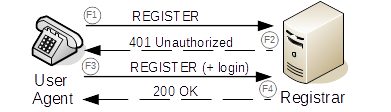
\includegraphics[width=\linewidth]{contents/background-in-isp-side-protocols/sip/sip-registration-flow.png}
    \caption{\gls{sip} Registration Flow}
    {Source: Korolev Alexandr}
    \label{figure:sip_register}
\end{figure}

Before making and receiving calls, the client must create a session by sending a REGISTER request to the \gls{sip} Registrar, shown on Figure \ref{figure:sip_register}. The server may request credentials with a challenge-response authentication mechanism, using the \gls{md5} algorithm \cite{rfc1321} by default.

\begin{figure}[h]
    \centering
    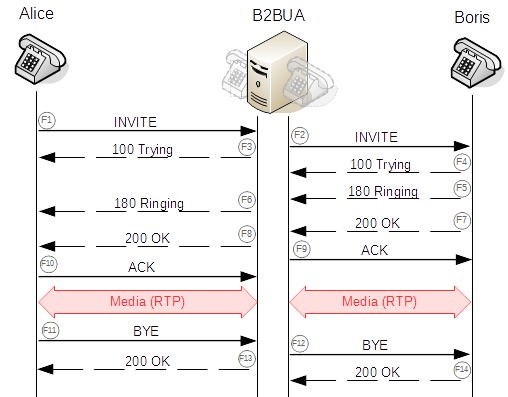
\includegraphics[width=\linewidth]{contents/background-in-isp-side-protocols/sip/sip-b2bua-call-flow.png}
    \caption{\gls{sip} Invitation Flow}
    {Source: Korolev Alexandr}
    \label{figure:sip_invite}
\end{figure}

With the session established, the client may invite another peer to a call through a \gls{sip} Proxy, the receiver is notified and may answer or decline the request. The invite carries all the mechanisms supported to communicate with the caller, leaving the callee to decide which one will be used upon acceptance. The procedure is represented in Figure \ref{figure:sip_invite}.

\FloatBarrier
